\documentclass[tikz,border=10pt]{standalone}
\usepackage{tkz-euclide} % 增强几何绘图功能
\usetikzlibrary{calc,intersections}

\begin{document}
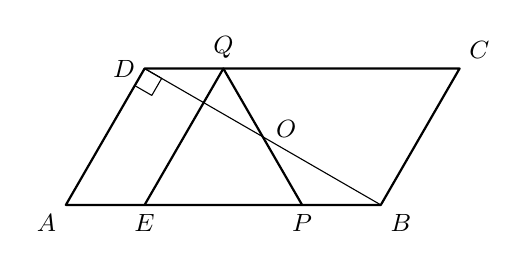
\begin{tikzpicture}[line join=round, line cap=round, >=stealth, font=\small]

    % --- 1. 定义核心顶点 (基于平行四边形结构) ---
    \coordinate (A) at (0,0);
    \coordinate (B) at (4,0);
    \coordinate (D) at (1,1.732);
    \coordinate (C) at ($(B)+(D)-(A)$); % 平行四边形顶点C

    % --- 2. 定义辅助点与线段 ---

    % 定义 P 点在 AB 上，Q 点在 CD 上
    \coordinate (P) at ($(A)!0.75!(B)$);
    \coordinate (Q) at ($(D)!0.25!(C)$);
    \coordinate (E) at ($(A)!0.25!(B)$);

    % 连接 BD
    \draw (B) -- (D);

    % --- 3. 绘制主轮廓 ---
    % 绘制平行四边形 ABCD
    \draw[thick] (A) -- (B) -- (C) -- (D) -- cycle;

    % 绘制三角形 EBC 的相关连线 (图中显示为 E-Q-B 结构)
    \draw[thick] (E) -- (Q);
    \draw[thick] (P) -- (Q);

    % 找到 PQ 与 BD 的交点 O
    \path [name path=PQ] (P) -- (Q);
    \path [name path=BD] (B) -- (D);
    \path [name intersections={of=PQ and BD, by=O}];

    % --- 4. 标注直角符号 ---
    % 根据图示，角 EDB 为直角
    \tkzMarkRightAngle[size=0.25](A,D,B)

    % --- 5. 绘制所有点和标签 ---
    

    % 打印标签
    \node [below left] at (A) {$A$};
    \node [below right] at (B) {$B$};
    \node [above right] at (C) {$C$};
    \node [left] at (D) {$D$};
    \node [below] at (E) {$E$};
    \node [below] at (P) {$P$};
    \node [above] at (Q) {$Q$};
    \node [shift={(0.3cm, 0.1cm)}] at (O) {$O$};

    % 可选：打点标记（如需要更明显的顶点）
    %\foreach \p in {A,B,C,D,E,P,Q,O} \fill (\p) circle (1pt);

\end{tikzpicture}
\end{document}